\documentclass[a4paper,conference]{IEEEtran}
\IEEEoverridecommandlockouts

% Essential LaTeX packages
\usepackage{cite}
\usepackage{amsmath,amssymb,amsfonts}
\usepackage{algorithmic}
\usepackage{graphicx}
\usepackage{textcomp}
\usepackage{xcolor}
\usepackage{booktabs}
\usepackage{multirow}
\usepackage{url}
\usepackage{microtype}

\usepackage{balance}

% Float control parameters for clean, professional IEEE conference layout
\renewcommand{\topfraction}{0.95}
\renewcommand{\bottomfraction}{0.95}
\renewcommand{\textfraction}{0.05}
\renewcommand{\floatpagefraction}{0.85}
\renewcommand{\dbltopfraction}{0.95}
\renewcommand{\dblfloatpagefraction}{0.85}

% Compact bibliography spacing
\def\IEEEbibitemsep{1pt plus 1pt}

\begin{document}

\title{An Explainable Machine Learning Framework for Phishing Website Detection Using URL and Network Features}

\author{
\IEEEauthorblockN{Tanay Samson Pathare}
\IEEEauthorblockA{Department of Computer Science, Bhonsala Military College\\
Nashik, Maharashtra, India\\
Email: tanaypathare1@gmail.com}
}

\maketitle

\begin{abstract}
Phishing websites represent a pervasive cyber threat engineered to harvest credentials through deceptive web infrastructure. While machine learning enables proactive detection beyond signature blacklists, operational deployment is hindered by model opacity and the latency of external domain inspection. This paper presents an explainable machine learning framework for phishing website detection using 111 structured URL lexical, path, query, and network resolver features on a benchmark corpus of 58,645 URLs. Evaluating five classification architectures across 11,729 held-out test instances with 5-fold cross-validation on the training set, XGBoost achieves superior discrimination, yielding 94.82\% accuracy and 95.05\% F1-score (5-seed mean: 94.74\% $\pm$ 0.08\% accuracy, 94.98\% $\pm$ 0.08\% F1-score), statistically outperforming Random Forest ($p < 0.001$, McNemar's test). Tree-based Shapley Additive Explanations (TreeSHAP) applied strictly to training data ensure train-only attribution, revealing high ranking stability under retraining and identifying directory length, domain registration age, and delimiters as primary discriminators. Feature reduction demonstrates that a compact top-20 subset—the smallest tested subset within 0.2\,pp of full training CV F1—preserves full test performance while lowering model inference latency to 1.67\,ms per 1,000 queries. Furthermore, an uncertainty-gated cascade resolves 64.3\% of URLs in-memory with 97.78\% accuracy using zero-network lexical parsing, establishing an operationally viable tiered triage architecture that eliminates nearly two-thirds of external resolver lookups.
\end{abstract}

\begin{IEEEkeywords}
Phishing Website Detection, Explainable Artificial Intelligence (XAI), Machine Learning, URL Features, TreeSHAP, Feature Selection, Cybersecurity.
\end{IEEEkeywords}

\section{Introduction}
\label{sec:intro}

Phishing represents a pervasive threat in modern cyberspace. Attackers engineer deceptive URLs and spoofed web portals to impersonate authentic organizations, harvesting credentials and financial assets. Threat telemetry from the Anti-Phishing Working Group (APWG) \cite{apwg2023trends} documents millions of active phishing attacks annually, while the Verizon Data Breach Investigations Report (DBIR) \cite{verizon2024dbir} identifies stolen credentials as a primary initial breach vector across thousands of confirmed corporate security incidents.

Conventional defenses rely heavily on centralized signature databases and community blacklists (e.g., Google Safe Browsing, PhishTank). While blacklists provide high precision on cataloged domains, they exhibit significant discovery delays, often requiring hours to verify zero-hour domains \cite{sahoo2017malicious, rao2019detection, hannousse2021towards, marchal2017off}, during which zero-day attacks achieve maximum impact.

To overcome blacklist latency, machine learning (ML) has emerged as a proactive alternative, classifying domain, path, and structural indicators dynamically \cite{sahingoz2019machine, babagoli2019heuristic}. However, operational adoption in Security Operations Centers (SOCs) faces two critical bottlenecks: (i) \textbf{Model Opacity}, where opaque tree ensembles fail to provide interpretable feature attributions for containment decisions; and (ii) \textbf{Page Crawling Latency}, where full DOM rendering introduces substantial latency and risks drive-by malware \cite{opara2020htmlphish, adebowale2023intelligent}.

To address these challenges, this paper presents an empirical benchmark and explainable ML framework for phishing detection using 111 structured URL lexical, path, file, query, and resolver metrics on 58,645 URLs \cite{vrbancic2020datasets}. We evaluate five paradigms: Logistic Regression, Decision Trees, Random Forests, Linear SVM, and XGBoost across 11,729 held-out test samples with 5-fold cross-validation. To ensure transparency, we apply Tree-based Shapley Additive Explanations (TreeSHAP) \cite{lundberg2020local, lundberg2017unified} strictly on training data to ensure train-only attribution.

The primary contributions of this work are:
\begin{itemize}
    \item \textbf{Multi-Model Benchmark \& Statistical Validation}: We evaluate five supervised ML architectures across 11,729 test instances with 5-fold CV on training data ($N=46,916$), verifying that XGBoost's lead (5-seed test mean: $94.74\% \pm 0.08\%$ accuracy, $94.98\% \pm 0.08\%$ F1; seed 42: 94.82\% accuracy, 95.05\% F1; seeds vary model tree subsampling on a fixed split) over Random Forest is statistically significant via McNemar's test ($p < 0.001$).
    \item \textbf{Train-Only Attribution \& Ranking Stability}: We implement TreeSHAP strictly on training data to ensure train-only attribution, demonstrating robust ranking stability under model retraining ($\rho_s = 0.973 \pm 0.010$ across all 98 features, Kendall's $\tau = 0.795$ within the top 20, and 95.0\% top-20 set overlap across independent model training seeds; $\rho_s = 0.9991$ and $\tau = 0.9131$ under explanation subsampling) and identifying primary signals (directory length, domain activation age, delimiters).
    \item \textbf{Feature Reduction \& Cascaded Triage}: We evaluate nested subsets, selecting $k=20$ as the smallest tested subset within about 0.2\,pp of full training CV F1, which sustains full test performance (5-seed test mean: $94.71\% \pm 0.09\%$ accuracy, $94.95\% \pm 0.08\%$ F1) while lowering model-only latency to $1.67$\,ms per 1,000 queries. Furthermore, evaluating an uncertainty-gated cascade demonstrates that a zero-network lexical-only model (84 features) resolves 64.3\% of URLs in-memory with 97.78\% Tier-1 accuracy, supporting a tiered design for high-throughput perimeter triage that offloads 64.3\% of external resolver queries while maintaining 94.57\% overall pipeline accuracy.
    \item \textbf{Computational Profiling}: We measure model inference latency (mean $\pm$ std over 20 repeated runs), single-query latency ($N=1$), serialized model footprints, and throughput under batched execution.
\end{itemize}

The remainder of this manuscript is organized as follows: Section~\ref{sec:related_work} surveys related work. Section~\ref{sec:methodology} presents the methodology. Section~\ref{sec:experiments} details the setup. Section~\ref{sec:results} discusses results. Section~\ref{sec:discussion} addresses trade-offs and error analysis. Section~\ref{sec:conclusion} concludes the paper.


\section{Related Work}
\label{sec:related_work}

The evolution of automated phishing detection spans four major paradigms: heuristic/blacklist methods, content-based deep learning, URL/network-based machine learning, and Explainable AI (XAI) frameworks.

\subsection{Heuristic and Blacklist-Based Detection}
Early defenses relied on signature repositories and community blacklists \cite{sahoo2017malicious}. While services like PhishTank and Google Safe Browsing provide authoritative verdicts for cataloged threats, studies by Hannousse and Yahiouche \cite{hannousse2021towards} and Marchal et al. \cite{marchal2017off} show that blacklists suffer from significant discovery latency. Attackers evade blacklists via domain generation algorithms (DGAs), fast-flux DNS, and disposable top-level domains (TLDs), enabling zero-day attacks to execute before signatures propagate.

\subsection{Content-Based and Deep Learning Approaches}
To overcome blacklist delays, several studies proposed inspecting web page contents, DOM trees, and scripts. Opara et al. \cite{opara2020htmlphish} developed \textit{HTMLPhish}, employing CNN-LSTM networks to analyze raw HTML document flows. Mohammad et al. \cite{mohammad2014predicting} investigated self-structuring neural networks on page-level features. Adebowale et al. \cite{adebowale2023intelligent} integrated convolutional and recurrent architectures on website features, while Al-Alyan and Al-Ahmadi \cite{alalyan2020robust} proposed a URL-only CNN trained on over two million URLs.

Despite high accuracy, content-based techniques exhibit significant practical liabilities: (i) they require live connections to hostile servers, risking malware execution; (ii) cloaking mechanisms serve benign decoys to crawlers; and (iii) fetching and rendering pages introduces heavy network and computational latency, preventing inline inspection.

\subsection{URL and Network-Centric Machine Learning}
To achieve high-throughput triage without page rendering, researchers turned toward feature engineering on URLs and network metadata. Sahoo et al. \cite{sahoo2017malicious} and Rao and Pais \cite{rao2019detection} established taxonomies of URL lexical properties. Sahingoz et al. \cite{sahingoz2019machine} evaluated tree classifiers and linear SVMs on lexical representations. Babagoli et al. \cite{babagoli2019heuristic} proposed heuristic non-linear regression strategies for phishing detection, while Chiew et al. \cite{chiew2019new} analyzed hybrid ensemble feature selection. Vrban{\v{c}}i{\v{c}} et al. \cite{vrbancic2020datasets} standardized a benchmark containing 111 structured features across 58,645 URLs, capturing URL, domain, directory, file, query, and resolver metadata without page rendering.

\subsection{Explainable Artificial Intelligence (XAI) in Cybersecurity}
Recent works have explored post-hoc interpretability in phishing detection. Al-Fayoumi et al. \cite{alfayoumi2024xaiphd} proposed \textit{XAI-PhD}, leveraging TreeSHAP with ensemble models to interpret URL classification decisions and prune features to reduce prediction overhead. Uddin et al. \cite{uddin2025explainable} combined gradient-boosting models with SHAP on a public Kaggle dataset. Calzarossa et al. \cite{calzarossa2024explainable} proposed an explainable machine learning procedure to identify critical phishing indicators, while Kehkashan et al. \cite{kehkashan2025explainable} evaluated random forest with SHAP on a Kaggle dataset of 11,000 URLs.

While these studies established the utility of post-hoc explanations, several methodological distinctions and gaps remain: (i) prior works in this domain, including XAI-PhD \cite{alfayoumi2024xaiphd}, do not explicitly specify whether global SHAP attributions and subsequent feature pruning are restricted strictly to an independent training partition or evaluated globally across the dataset prior to final validation, a practice that risks subtle selection leakage if test instances inform feature pruning; (ii) attribution ranking stability across random seeds and subsamples is often unquantified; (iii) existing feature selection methods treat all features uniformly, whereas in practice, synchronous external network lookups (DNS/WHOIS) incur tens to hundreds of milliseconds of latency compared to microsecond in-memory lexical parsing; and (iv) computational latency reporting frequently omits repeated measurement intervals or single-query benchmarking. This paper addresses these challenges by enforcing a strict train-only TreeSHAP protocol on the standardized 58,645 URL corpus \cite{vrbancic2020datasets}, verifying attribution stability across seeds, and evaluating an uncertainty-gated cascade that explicitly decouples in-memory lexical parsing from network resolver queries.


\section{Proposed Methodology}
\label{sec:methodology}

The architectural pipeline of the proposed framework is illustrated in Fig.~\ref{fig:architecture}. It operates across four stages: (i) static feature extraction and zero-variance filtering, (ii) multi-model supervised classification, (iii) train-only TreeSHAP feature attribution on training data, and (iv) SHAP-directed feature pruning and computational profiling.

\begin{figure}[htbp]
\centering
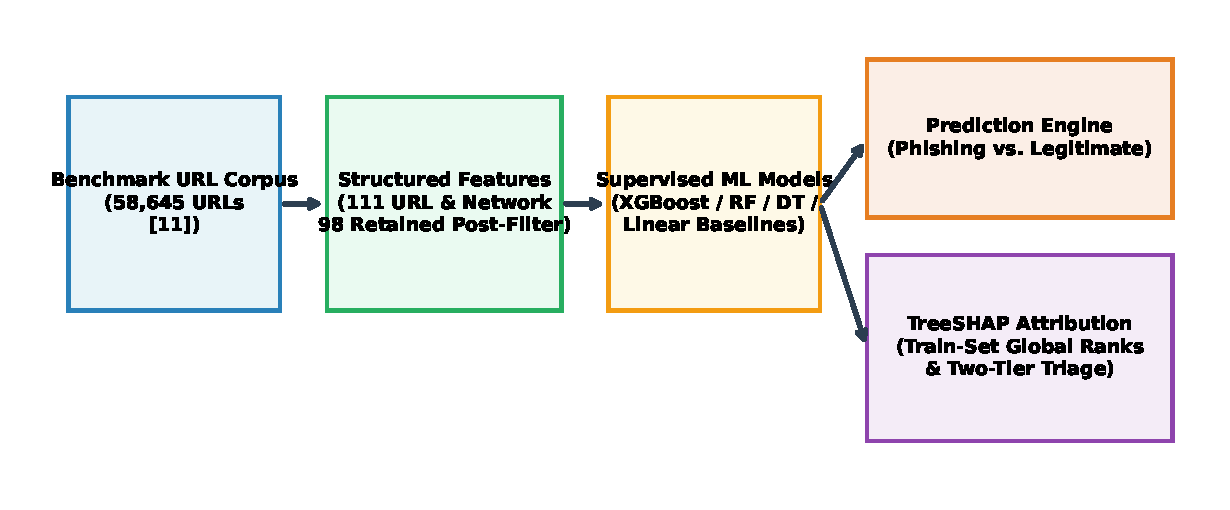
\includegraphics[width=0.88\columnwidth]{figures/fig1_system_architecture.pdf}
\caption{Architectural Pipeline of the Proposed Explainable Phishing Detection Framework.}
\label{fig:architecture}
\end{figure}

\subsection{Dataset Formulation and Preprocessing}
We utilize the benchmark dataset curated by Vrban{\v{c}}i{\v{c}} et al. \cite{vrbancic2020datasets}, containing 58,645 URLs (30,647 phishing from PhishTank/OpenPhish and 27,998 legitimate from Alexa top sites, search results, and open community directories). Table~\ref{tab:dataset} outlines the dataset parameters.

\begin{table}[htbp]
\caption{Dataset Specification and Partitioning}
\label{tab:dataset}
\centering
\resizebox{\columnwidth}{!}{
\begin{tabular}{lp{4.5cm}}
\hline
\textbf{Property} & \textbf{Specification / Value} \\
\hline
Dataset Provenance & Vrban\v{c}i\v{c} et al. (\textit{Data in Brief}, 2020) \cite{vrbancic2020datasets} \\
Feature Modality & Static URL Lexical, Path, File, Query, and Resolver \\
Total URL Instances & 58,645 URLs \\
Raw Feature Dimensions & 111 Numeric Features (97 Lexical / 14 Resolver; 96/15 in \cite{vrbancic2020datasets}) \\
Retained Dimensions & 98 Informative Features (13 Constant Domain Delimiters Filtered) \\
Target Class & Binary: Phishing (1) vs. Legitimate (0) \\
Phishing Instances & 30,647 (52.26\%) \\
Legitimate Instances & 27,998 (47.74\%) \\
Train / Test Partition & 80\% Stratified Train (46,916) / 20\% Test (11,729) \\
Missing / Sentinel Values & 0 NaN (Unset/unavailable metrics encoded as $-1$) \\
\hline
\end{tabular}
}
\end{table}


\begin{figure}[htbp]
\centering
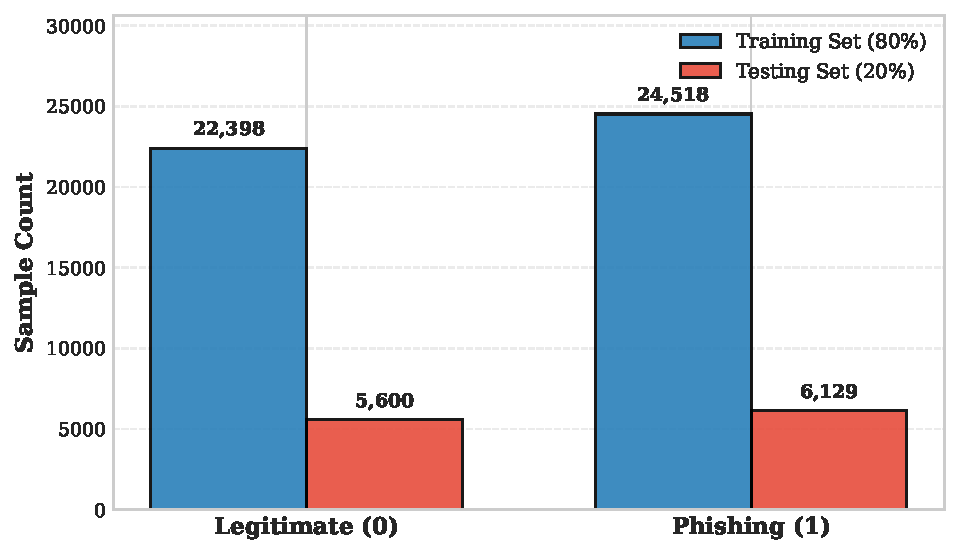
\includegraphics[width=0.88\columnwidth]{figures/fig2_class_distribution.pdf}
\caption{Class distribution across stratified train (80\%) and test (20\%) partitions.}
\label{fig:class_dist}
\end{figure}

As shown in Fig.~\ref{fig:class_dist}, the dataset is partitioned into an 80\% training corpus ($N_{\text{train}} = 46,916$) and a 20\% held-out test corpus ($N_{\text{test}} = 11,729$) using stratified sampling to preserve the 52.26\% : 47.74\% class distribution across partitions. Let $\mathcal{D} = \{(\mathbf{x}_i, y_i)\}_{i=1}^N$ denote the dataset, where $\mathbf{x}_i \in \mathbb{R}^D$ ($D=111$) and $y_i \in \{0, 1\}$. 

A cross-partition feature vector audit reveals that across the 98 retained features, exactly 335 test instances (2.86\% of the 11,729 test set) share identical feature vectors with instances in the training set. Within partitions, 906 rows in train (1.93\%) and 130 rows in test (1.11\%) represent internal duplicates. This occurs because distinct root-level URLs that lack path/query strings and share common registrar or default $-1$ values collapse to identical discrete feature vectors. Crucially, 332 of the 335 cross-partition twin pairs (99.1\%) share identical ground-truth labels (with only 3 label conflicts, 0.9\%). Evaluating on the strictly de-duplicated test subset ($N = 11,394$, where all 335 cross-partition twins are removed), XGBoost achieves 94.71\% accuracy and 95.05\% F1-score, while Random Forest achieves 94.18\% accuracy and 94.58\% F1-score (compared to 94.82\% / 95.05\% and 94.30\% / 94.57\% on the full test set), verifying that cross-partition repetition does not inflate generalization metrics.

A fundamental structural characteristic of this dataset is the use of the numeric sentinel $-1$ to denote ``not applicable'' or ``lookup unavailable'' (e.g., URLs lacking directory paths or query strings assign $-1$ to path/query metrics, and failed/unresolved WHOIS lookups assign $-1$ to activation age). This design preserves complete matrix density while encoding structural absence. Preprocessing fits a zero-variance filter $\mathcal{V}(X_j) = \frac{1}{N_{\text{train}}} \sum_{i=1}^{N_{\text{train}}} (x_{ij} - \mu_j)^2 > 0$ strictly on $\mathcal{D}_{\text{train}}$. Thirteen constant features (all belonging to the domain structural family) are eliminated, leaving $D' = 98$ informative features (84 lexical/structural and 14 network/resolver metrics). For distance-based models (Logistic Regression and Linear SVM), features are standardized via z-score scaling $z_{ij} = (x_{ij} - \mu_j)/\sigma_j$ fitted exclusively on $\mathcal{D}_{\text{train}}$.

\subsection{URL Feature Engineering Taxonomy}
The 111 structured metrics span six cybersecurity feature families ($20 + 21 + 18 + 18 + 20 + 14 = 111$ raw; $20 + 8 + 18 + 18 + 20 + 14 = 98$ retained). In the original benchmark specification \cite{vrbancic2020datasets}, the authors report 96 features extracted directly from URL strings and 15 extracted via custom Python logic (consisting of 14 external resolver metrics alongside \texttt{email\_in\_url}). In our framework, \texttt{email\_in\_url} is classified as an in-memory URL lexical metric because regex checking for an email pattern within a raw URL string requires zero external network queries or socket handshakes. Thus, we delineate 97 lexical/structural features (84 retained) and 14 external resolver features:
\begin{enumerate}
    \item \textbf{URL Lexical} (20/20 retained): URL character length (\texttt{length\_url}), presence flags (\texttt{email\_in\_url}), and delimiter frequencies (\texttt{qty\_slash\_url}, \texttt{qty\_dot\_url}, \texttt{qty\_hyphen\_url}, \texttt{qty\_equal\_url}, \texttt{qty\_and\_url}).
    \item \textbf{Domain Structural} (21/8 retained): Domain string length (\texttt{domain\_length}), IP indicator (\texttt{domain\_in\_ip}), authority dots (\texttt{qty\_dot\_domain}), vowels, and hyphens. Thirteen zero-variance domain delimiters (e.g., slashes, question marks, and symbols within domain authority) are eliminated.
    \item \textbf{Directory/Path} (18/18 retained): Directory character length (\texttt{directory\_length}), slash count (\texttt{qty\_slash\_directory}), and path delimiters (encoded as $-1$ when no directory is present).
    \item \textbf{File-Level} (18/18 retained): Filename length (\texttt{file\_length}) and character counts.
    \item \textbf{Query/Parameter} (20/20 retained): Query length (\texttt{params\_length}), parameter count (\texttt{qty\_params}), and argument delimiters.
    \item \textbf{Resolver/Network} (14/14 retained): Passive and active external lookups and search indicators: HTTP response latency (\texttt{time\_response}), SPF record flag (\texttt{domain\_spf}), Autonomous System Number (\texttt{asn\_ip}), domain activation age (\texttt{time\_domain\_activation}), domain expiration time (\texttt{time\_domain\_expiration}), resolved IP count (\texttt{qty\_ip\_resolved}), authoritative nameserver count (\texttt{qty\_nameservers}), MX mail server count (\texttt{qty\_mx\_servers}), DNS TTL (\texttt{ttl\_hostname}), TLS/SSL certificate status (\texttt{tls\_ssl\_certificate}), redirect hop count (\texttt{qty\_redirects}), URL Google index status (\texttt{url\_google\_index}), domain Google index status (\texttt{domain\_google\_index}), and URL shortener lookup flag (\texttt{url\_shortened}). Filtering 13 constant domain delimiters leaves exactly 84 purely in-memory lexical and structural features across groups 1--5 that require strictly 0 external network lookups.
\end{enumerate}

\subsection{Classification Model Architectures}
We evaluate five diverse classification paradigms: (i) \textbf{Logistic Regression (LR)} with L2 regularization ($C=1.0$); (ii) \textbf{Decision Trees (DT)} with Gini impurity splitting ($\text{max\_depth}=12$); (iii) \textbf{Random Forest (RF)} ensemble with 100 bagging trees ($\text{max\_depth}=15$); (iv) \textbf{Linear SVM} with Platt calibration; and (v) \textbf{XGBoost} \cite{chen2016xgboost} (100 estimators, $\text{max\_depth}=6$, $\eta=0.1$, subsample=0.8, colsample=0.8), minimizing the regularized objective: $\mathcal{L}^{(t)} = \sum_{i=1}^N l\left(y_i, \hat{y}_i^{(t-1)} + f_t(\mathbf{x}_i)\right) + \gamma T + \frac{1}{2}\lambda \sum_{j=1}^T w_j^2$. Table~\ref{tab:model_config} lists the detailed hyperparameters.

\begin{table}[htbp]
\caption{Model Hyperparameter Configurations}
\label{tab:model_config}
\centering
\resizebox{\columnwidth}{!}{
\begin{tabular}{lp{4.5cm}}
\hline
\textbf{Model Architecture} & \textbf{Hyperparameter Specification} \\
\hline
Logistic Regression & L2 penalty, $C=1.0$, L-BFGS solver, max\_iter=1000 \\
Decision Tree & Gini impurity, max\_depth=12, min\_samples\_split=10 \\
Random Forest & 100 trees, max\_depth=15, min\_samples\_split=5 \\
Linear SVM & LinearSVC ($C=1.0$), Platt calibrated (3-fold CV) \\
XGBoost & 100 estimators, max\_depth=6, $\eta=0.1$, subsample=0.8, colsample=0.8, histogram method \\
\hline
\end{tabular}
}
\end{table}


\subsection{Explainable AI via TreeSHAP}
To explain model decisions, we deploy TreeSHAP \cite{lundberg2020local, lundberg2017unified}, which satisfies the additive attribution property $f(\mathbf{x}) = \phi_0 + \sum_{j=1}^{D'} \phi_j(\mathbf{x})$, where $\phi_0 = \mathbb{E}[f(\mathbf{x})]$ is the expected base model output, and $\phi_j(\mathbf{x})$ is the Shapley attribution:
\begin{equation}
\phi_j(\mathbf{x}) = \sum_{\mathcal{S} \subseteq \mathcal{F} \setminus \{j\}} \frac{|\mathcal{S}|! (|\mathcal{F}| - |\mathcal{S}| - 1)!}{|\mathcal{F}|!} \left[ f(\mathcal{S} \cup \{j\}) - f(\mathcal{S}) \right]
\label{eq:shap_formula}
\end{equation}

Global feature importance $I_j$ is computed as the mean absolute SHAP value strictly over a training explanation subset $\mathcal{X}_{\text{train, exp}} \subset \mathcal{D}_{\text{train}}$ ($N=500$ random samples): $I_j = \frac{1}{|\mathcal{X}_{\text{train, exp}}|} \sum_{i \in \mathcal{X}_{\text{train, exp}}} |\phi_j(\mathbf{x}_i)|$. Deriving $I_j$ exclusively on $\mathcal{D}_{\text{train}}$ establishes train-only attribution and prevents selection leakage into feature selection. Under model retraining across independent seeds (varying tree subsampling), global feature rankings demonstrate high stability: $\rho_s = 0.973 \pm 0.010$ Spearman rank correlation across all 98 features, Kendall's $\tau = 0.7948 \pm 0.031 \approx 0.79$ within the top-20 features, and 95.0\% top-20 set overlap (19 of 20 features preserved across all retrained models). When fixing the model and varying only the explanation subsampling seed, rankings show near-perfect agreement ($\rho_s = 0.9991$, Pearson $r = 0.9995$, Kendall's $\tau = 0.9131$ within top-20, 100\% top-20 set overlap; $\rho_s = 0.9995$ between $N=500$ and $N=1,000$), confirming that high stability is robust and not an artifact of tied near-zero features in the tail. Ranked features $I_{(1)} \ge I_{(2)} \ge \dots \ge I_{(D')}$ direct nested feature pruning.


\section{Experimental Setup}
\label{sec:experiments}

\subsection{Implementation and Computational Environment}
All experiments are implemented in Python 3.14 utilizing \texttt{scikit-learn} (v1.9.1), \texttt{xgboost} (v3.4.1), \texttt{shap} (v0.52.0), and \texttt{scipy} (v1.18.1). Execution was conducted on an x86\_64 Linux environment equipped with an Intel Core i5-3337U processor @ 1.80\,GHz (2 physical cores, 4 threads) and 4\,GB physical RAM running Ubuntu Linux. Random seed 42 is fixed across data partitioning, cross-validation folds, and subsampling for deterministic reproducibility, with multi-seed evaluations (seeds 42, 123, 456, 789, 2024; which retrain models to vary tree subsampling on the fixed test split) validating variance bounds. Hyperparameters are held at fixed baseline configurations (Table~\ref{tab:model_config}) to evaluate architectural efficacy.

\subsection{Evaluation Metrics and Validation Protocols}
To evaluate detection efficacy on the binary classification task ($1 = \text{Phishing}$, $0 = \text{Legitimate}$), we calculate standard performance metrics: $\text{Accuracy} = \frac{TP + TN}{TP + TN + FP + FN}$, $\text{Precision} = \frac{TP}{TP + FP}$, $\text{Recall} = \frac{TP}{TP + FN}$, $\text{F1-Score} = \frac{2 \times \text{Precision} \times \text{Recall}}{\text{Precision} + \text{Recall}}$, $\text{FPR} = \frac{FP}{FP + TN}$, and $\text{FNR} = \frac{FN}{FN + TP}$, alongside continuous probability diagnostics (ROC-AUC and Average Precision PR-AUC).

Generalization stability is evaluated using 5-Fold Stratified Cross-Validation on the training partition ($N_{\text{train}} = 46,916$), recording the mean $\pm$ standard deviation across folds. Crucially, to prevent data leakage across validation folds, zero-variance feature filtering and standard scaling transformations are fitted strictly within each training fold pipeline rather than globally prior to cross-validation. Furthermore, to avoid test-set reuse in feature selection, candidate subset dimensions were evaluated by 5-fold CV on $\mathcal{D}_{\text{train}}$, selecting $k=20$ as the smallest tested subset within about 0.2 percentage points of full performance (CV F1: 91.85\% at $k=5$, 94.52\% at $k=10$, 95.02\% at $k=20$, 95.17\% at $k=30$, and 95.20\% at $k=98$). Because global SHAP rankings were derived across all of $\mathcal{D}_{\text{train}}$, cross-validation scores for the top-$k$ subsets are slightly optimistic due to feature selection on the full training pool; however, held-out test evaluations remain strictly unaffected. Both Table~\ref{tab:model_comparison} and the $k$-sweep utilize identical 5-fold stratified cross-validation splits and preprocessing pipelines; full-model CV F1 records $95.17\% \pm 0.13\%$ in the multi-model benchmark (evaluated with histogram-based tree splitting, \texttt{tree\_method="hist"}) and $95.20\% \pm 0.17\%$ in the standalone $k$-sweep (evaluated under standard exact tree construction), demonstrating cross-validation stability within 0.03\,pp across splitting routines. Final model evaluation is performed on the untouched held-out test partition ($N_{\text{test}} = 11,729$). Statistical significance between classifier predictions is verified using McNemar's test with Edwards continuity correction.

\subsection{Computational Benchmarking Protocol}
Model inference latency is measured in batched vector mode over the entire held-out test matrix ($N=11,729$) using \texttt{predict()} with multi-threading enabled (\texttt{n\_jobs=-1}). To eliminate cold-start caching artifacts, each model executes two warm-up passes followed by 20 repeated measurement iterations. Latency is standardized as milliseconds per 1,000 queries ($\text{ms} / 10^3\,\text{URLs}$), reporting mean $\pm$ standard deviation. In addition, to account for single-threaded runtime differences across linear and tree models under unbatched stream deployment, we benchmark single-query latency ($N=1$, batch size 1) across 500 repeated trials (Decision Tree: 0.22\,ms, Logistic Regression: 0.30\,ms, XGBoost: 0.71\,ms, Linear SVM: 4.01\,ms, Random Forest: 49.38\,ms; compact Top-20 XGBoost: 0.46\,ms median, 0.56\,ms mean). XGBoost's single-query latency (0.71\,ms) is approximately 60$\times$ the 11.6\,$\mu$s required for in-memory lexical feature extraction; we note that this latency reflects Python interpreter and object conversion overhead, and production deployment via native compiled runtimes (e.g., Treelite or C++ ONNX) can reduce single-query latency into microseconds. Storage footprint is measured by serializing fitted model structures using \texttt{joblib} (compression level 3). In-memory string-based feature extraction speed is benchmarked over 10,000 raw URL string parsing operations (extracting all 84 retained lexical properties including character counts, token delimiters, and structural lengths across URL, domain authority, directory path, filename, and query parameter components in pure CPU memory without I/O), yielding an average extraction latency of 11.6\,$\mu$s per URL (11.6\,ms per $10^3$ URLs).


\section{Results and Empirical Analysis}
\label{sec:results}

\subsection{Comparative Classifier Performance}
Table~\ref{tab:model_comparison} summarizes the empirical performance of all five machine learning models on the held-out test partition ($N_{\text{test}} = 11,729$), alongside 5-fold cross-validation scores on the training set, PR-AUC, and batched inference latency.

\begin{table*}[t]
\caption{Classification Performance and Computational Latency Across Evaluated ML Models (Test Set: $N=11,729$)}
\label{tab:model_comparison}
\centering
\resizebox{\textwidth}{!}{
\begin{tabular}{lccccccccc}
\hline
\textbf{Model Architecture} & \textbf{Acc (\%)} & \textbf{Prec (\%)} & \textbf{Rec (\%)} & \textbf{F1 (\%)} & \textbf{ROC-AUC} & \textbf{PR-AUC (AP)} & \textbf{5-Fold CV F1 (\%)} & \textbf{Batch Lat (ms per 1,000 URLs)} & \textbf{Single Lat (ms)} \\
\hline
Logistic Regression & 89.97 & 89.23 & 91.91 & 90.55 & 0.9613 & 0.9637 & 90.48 $\pm$ 0.20 & 1.41 $\pm$ 0.16 & 0.30 \\
Decision Tree & 93.61 & 93.36 & 94.49 & 93.92 & 0.9668 & 0.9546 & 93.62 $\pm$ 0.17 & 0.53 $\pm$ 0.05 & 0.22 \\
Random Forest & 94.30 & 94.03 & 95.12 & 94.57 & 0.9867 & 0.9880 & 94.79 $\pm$ 0.11 & 10.60 $\pm$ 0.31 & 49.38 \\
Linear SVM & 89.99 & 89.10 & 92.12 & 90.58 & 0.9613 & 0.9637 & 90.45 $\pm$ 0.22 & 2.85 $\pm$ 0.20 & 4.01 \\
\textbf{XGBoost} & \textbf{94.82} & \textbf{94.88} & \textbf{95.22} & \textbf{95.05} & \textbf{0.9879} & \textbf{0.9889} & \textbf{95.17 $\pm$ 0.13} & \textbf{2.46 $\pm$ 0.20} & \textbf{0.71} \\
\hline
\multicolumn{10}{l}{\footnotesize * PR-AUC corresponds to Average Precision (AP). Multi-seed XGBoost evaluation (5 random seeds) yields $94.74\% \pm 0.08\%$ Acc and $94.98\% \pm 0.08\%$ F1.} \\
\end{tabular}
}
\end{table*}


Tree-based ensemble architectures demonstrate superior discriminative capability over linear baselines:
\begin{itemize}
    \item \textbf{XGBoost} achieves the highest overall performance: 94.82\% Accuracy, 94.88\% Precision, 95.22\% Recall, 95.05\% F1, 0.9879 ROC-AUC, and 0.9889 PR-AUC (5-fold CV F1: $95.17\% \pm 0.13\%$) with $2.46 \pm 0.20$\,ms batch latency per $10^3$ URLs and 0.71\,ms single-query latency ($\sim 60\times$ the 11.6\,$\mu$s feature extraction time).
    \item \textbf{Random Forest} attains 94.30\% Accuracy, 94.57\% F1, 0.9867 ROC-AUC, and 0.9880 PR-AUC (CV F1: $94.79\% \pm 0.11\%$) with $10.60 \pm 0.31$\,ms latency per $10^3$ URLs.
    \item \textbf{Decision Tree} achieves 93.61\% Accuracy, 93.92\% F1, and 0.9668 ROC-AUC (CV F1: $93.62\% \pm 0.17\%$) at $0.53 \pm 0.05$\,ms latency.
    \item \textbf{Linear Models} (Logistic Regression and Linear SVM) attain 89.97\% and 89.99\% accuracy (CV F1: $90.48\%$ and $90.45\%$). Both models produce near-identical ROC-AUC (0.9613) and PR-AUC (0.9637) when rounded to four decimals (unrounded: 0.961327 vs. 0.961293 ROC-AUC; 0.963710 vs. 0.963676 PR-AUC). This parity is directly substantiated by the high cosine similarity of their standardized coefficient vectors ($\cos(\mathbf{w}_{\text{LR}}, \mathbf{w}_{\text{SVM}}) = 0.8307$) and a near-unity rank correlation between their continuous test decision scores ($\rho_s = 0.9997$ Spearman rank correlation, Pearson $r = 0.9836$); because threshold-free ROC and PR curves depend strictly on the rank-ordering of prediction scores, near-identical test rankings generate identical rounded area metrics.
\end{itemize}

On the test set, XGBoost identifies 5,836 True Positives ($TP$) out of 6,129 phishing URLs ($\text{Recall} = 95.22\%$) and 5,285 True Negatives ($TN$) out of 5,600 benign URLs ($\text{Specificity} = 94.38\%$), with $\text{FPR} = 5.62\%$ and $\text{FNR} = 4.78\%$.

To verify whether XGBoost's performance advantage over Random Forest is statistically significant, we conducted McNemar's test with continuity correction on test predictions ($b=161$ instances where XGBoost was correct and RF incorrect; $c=100$ instances where RF was correct and XGBoost incorrect). The test yields $\chi^2 = 13.79$ ($p = 2.04 \times 10^{-4} < 0.001$), confirming statistical significance. Multi-seed evaluation across 5 random seeds (seeds 42, 123, 456, 789, 2024; varying model tree subsampling with fixed test split) confirms stability: XGBoost achieves a mean accuracy of $94.74\% \pm 0.08\%$ and a mean F1-score of $94.98\% \pm 0.08\%$ versus Random Forest's $94.59\% \pm 0.06\%$.

\begin{figure}[htbp]
\centering
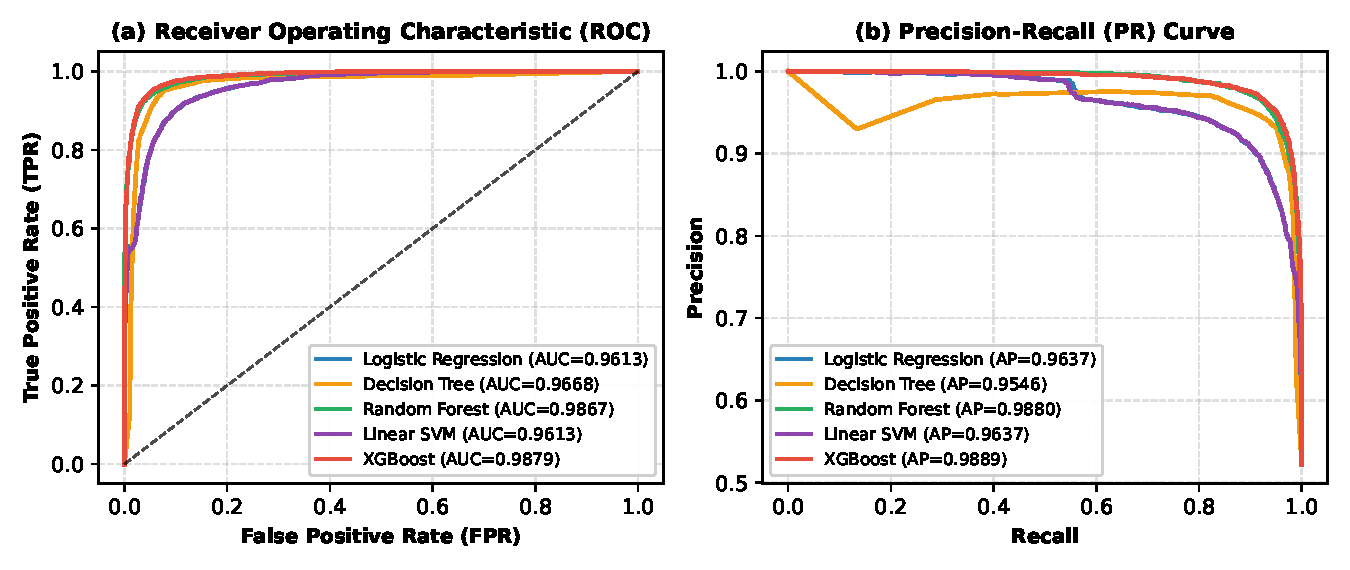
\includegraphics[width=0.88\columnwidth]{figures/fig5_roc_pr_curves.pdf}
\caption{Discrimination Diagnostics: (a) ROC Curves, and (b) Precision-Recall Curves across all evaluated classifiers.}
\label{fig:roc_pr}
\end{figure}

Fig.~\ref{fig:roc_pr} depicts the ROC and Precision-Recall (PR) curves. XGBoost and Random Forest maintain steep true positive trajectories, achieving Average Precision (AP) scores of 0.9889 and 0.9880 respectively, with Decision Tree achieving 0.9546 AP.

\subsection{Explainable AI via TreeSHAP}
TreeSHAP analysis was executed strictly on the training partition ($N=500$ random samples) to extract global feature rankings under a train-only protocol. Table~\ref{tab:shap_features} details the top 10 most influential features according to mean absolute SHAP value and plausible cybersecurity semantic rationales.

\begin{table*}[t]
\caption{Top 10 Most Influential Features Ranked by Mean Absolute TreeSHAP Value on Training Partition}
\label{tab:shap_features}
\centering
\begin{tabular}{clccp{10.5cm}}
\hline
\textbf{Rank} & \textbf{Feature Identifier} & \textbf{Modality} & \textbf{Mean $|\text{SHAP}|$} & \textbf{Plausible Cybersecurity Interpretation} \\
\hline
1 & \texttt{directory\_length} & Lexical & 1.0811 & Directory path length / presence (deep nesting often masks fraud; $-1$ indicates no path) \\
2 & \texttt{time\_domain\_activation} & Network & 0.9912 & Domain age in days (new domains and failed lookups often correlate with throwaway setups) \\
3 & \texttt{qty\_slash\_url} & Lexical & 0.7377 & Forward slash delimiter count across URL hierarchy \\
4 & \texttt{length\_url} & Lexical & 0.7222 & Raw URL character length (often used to obscure destination) \\
5 & \texttt{qty\_dot\_domain} & Lexical & 0.5293 & Subdomain dot count (frequently used in multi-level brand spoofing) \\
6 & \texttt{ttl\_hostname} & Network & 0.3147 & DNS TTL metric (short TTLs are consistent with fast-flux evasive DNS) \\
7 & \texttt{asn\_ip} & Network & 0.2057 & Autonomous System Number (differentiates bulletproof/rogue hosting ASNs) \\
8 & \texttt{time\_response} & Network & 0.1724 & HTTP response latency in seconds (reflects temporary host variability) \\
9 & \texttt{qty\_hyphen\_directory} & Lexical & 0.1277 & Hyphens in directory path (often inserted to mimic brand keywords) \\
10 & \texttt{qty\_redirects} & Network & 0.1082 & HTTP redirection hop count (multi-hop chains obscure destination landing) \\
\hline
\end{tabular}
\end{table*}


\begin{figure}[htbp]
\centering
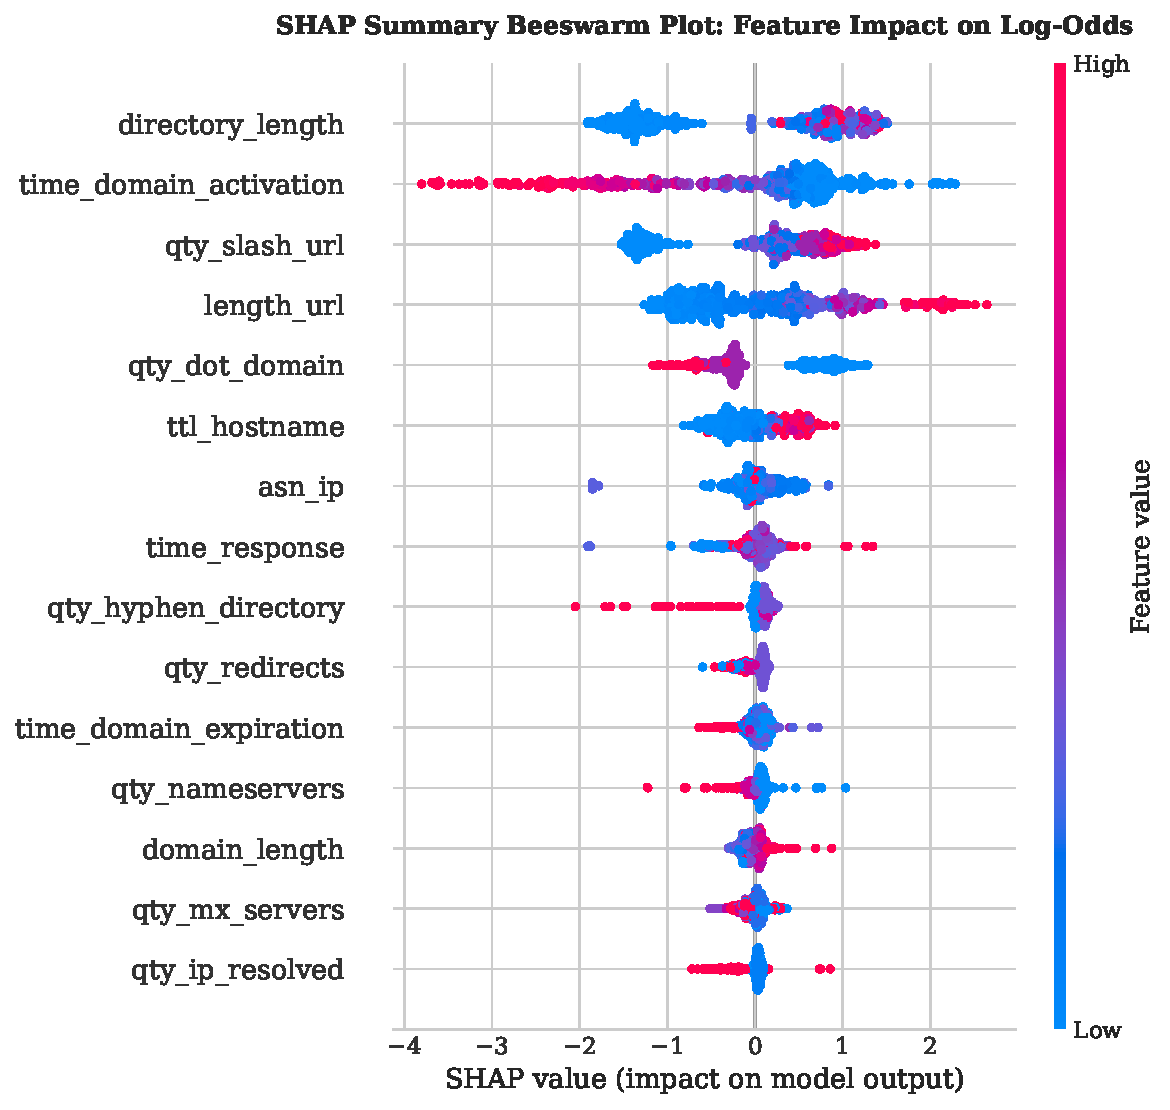
\includegraphics[width=0.88\columnwidth]{figures/fig7_shap_summary_beeswarm.pdf}
\caption{SHAP Summary Beeswarm Plot Illustrating Feature Impact Directionality on the Training Partition.}
\label{fig:shap_beeswarm}
\end{figure}

Fig.~\ref{fig:shap_beeswarm} illustrates global importance and directional attribution across training samples:
\begin{enumerate}
    \item \textbf{Directory Length (\texttt{directory\_length})}: Emerges as the top feature ($\text{Mean } |\text{SHAP}| = 1.0811$). Elongated paths (red points) shift predictions toward higher phishing log-odds. Crucially, as detailed in Section~\ref{sec:methodology}, this attribution reflects both directory depth and qualitative presence, as 60.29\% of legitimate test URLs (59.86\% in the training partition) lack paths (encoded as $-1$). Decision trees split between $-1$ (path absent) and positive lengths, effectively combining existence and magnitude into a single decision threshold.
    \item \textbf{Domain Registration Age (\texttt{time\_domain\_activation})}: Represents the second most decisive feature ($0.9912$). Mature domains correlate with negative SHAP values (legitimate signal), whereas recent domains and unresolvable WHOIS records ($-1$ sentinels) shift log-odds toward phishing, capturing throwaway infrastructure.
    \item \textbf{Delimiters and Structural Tokens (\texttt{qty\_slash\_url}, \texttt{length\_url}, \texttt{qty\_dot\_domain})}: Slash counts ($0.7377$), URL length ($0.7222$), and authority dots ($0.5293$) reflect structural obfuscation tactics commonly leveraged to evade token filters.
\end{enumerate}

\subsection{Feature Selection and Computational Benchmarking}
To assess whether compact feature subsets maintain classification performance, we evaluated XGBoost across nested feature subsets ranked by training set SHAP importance: Full (98 features), Top-30, Top-20, Top-10, Top-5, alongside a dedicated \textbf{Lexical-Only baseline} (84 features, 0 network lookups). Table~\ref{tab:feature_selection_resources} and Fig.~\ref{fig:feature_selection} delineate performance, latency, and throughput trade-offs.

\begin{table*}[t]
\caption{Impact of Feature Reduction and Computational Profile (Test Set: $N=11,729$)}
\label{tab:feature_selection_resources}
\centering
\resizebox{\textwidth}{!}{
\begin{tabular}{lccccccr}
\hline
\textbf{Configuration} & \textbf{Net / Lex} & \textbf{Acc (\%)} & \textbf{F1 (\%)} & \textbf{ROC-AUC} & \textbf{Lat (ms / $10^3$ URLs)} & \textbf{Size (MB)} & \textbf{Throughput (q/s)} \\
\hline
XGBoost (Full 98) & 14N / 84L & 94.82 & 95.05 & 0.9879 & 2.46 $\pm$ 0.20 & 0.126 & 406,318 \\
XGBoost (Top-30) & 12N / 18L & 94.74 & 94.97 & 0.9882 & 1.83 $\pm$ 0.07 & 0.134 & 546,448 \\
\textbf{XGBoost (Top-20)} & \textbf{11N / 9L} & \textbf{94.82} & \textbf{95.05} & \textbf{0.9876} & \textbf{1.67 $\pm$ 0.06} & \textbf{0.130} & \textbf{600,099} \\
XGBoost (Top-10) & 5N / 5L & 94.19 & 94.48 & 0.9859 & 1.57 $\pm$ 0.11 & 0.126 & 636,942 \\
XGBoost (Top-5) & 1N / 4L & 91.32 & 91.84 & 0.9723 & 1.59 $\pm$ 0.12 & 0.121 & 628,930 \\
\textbf{XGBoost (Lexical-84)} & \textbf{0N / 84L} & \textbf{89.68} & \textbf{90.04} & \textbf{0.9627} & \textbf{3.16 $\pm$ 0.43} & \textbf{0.342} & \textbf{316,002} \\
\hline
Random Forest & 14N / 84L & 94.30 & 94.57 & 0.9867 & 10.60 $\pm$ 0.31 & 4.068 & 94,369 \\
Decision Tree & 14N / 84L & 93.61 & 93.92 & 0.9668 & 0.53 $\pm$ 0.05 & 0.029 & 1,884,868 \\
Linear SVM & 14N / 84L & 89.99 & 90.58 & 0.9613 & 2.85 $\pm$ 0.20 & 0.006 & 350,920 \\
Logistic Regression & 14N / 84L & 89.97 & 90.55 & 0.9613 & 1.41 $\pm$ 0.16 & 0.004 & 708,898 \\
\hline
\multicolumn{8}{l}{\footnotesize * Evaluated under random seed 42. Multi-seed test evaluation for Top-20 (5 seeds) yields $94.71\% \pm 0.09\%$ Acc and $94.95\% \pm 0.08\%$ F1.} \\
\end{tabular}
}
\end{table*}


\begin{figure}[htbp]
\centering
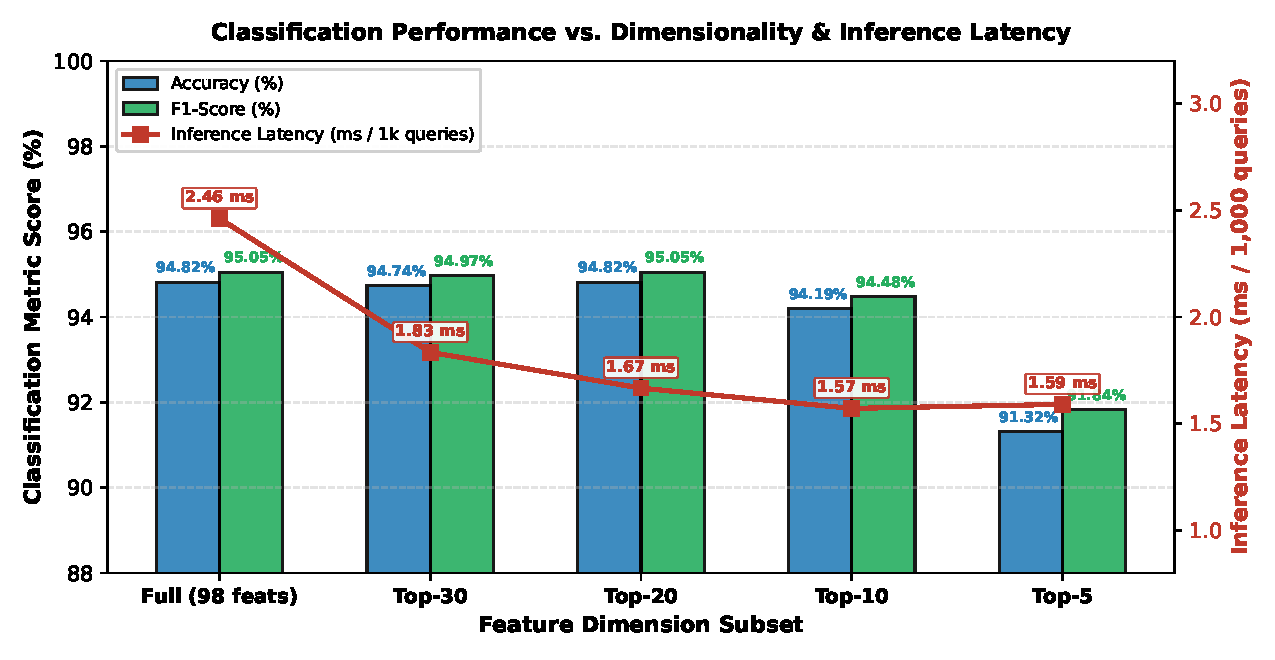
\includegraphics[width=0.88\columnwidth]{figures/fig9_feature_reduction_comparison.pdf}
\caption{Classification Performance vs. Dimensionality and Inference Latency Across Feature Subsets.}
\label{fig:feature_selection}
\end{figure}

Evaluating nested feature reduction via 5-fold cross-validation on $\mathcal{D}_{\text{train}}$ reveals progressive convergence: CV F1 increases from 91.85\% at $k=5$ and 94.52\% at $k=10$ to 95.02\% at $k=20$, 95.17\% at $k=30$, and 95.20\% at $k=98$. Although CV performance continues to edge upward at higher dimensions, we select $k=20$ as the smallest tested subset within about 0.2\,pp of full performance. Because SHAP feature rankings were computed on all of $\mathcal{D}_{\text{train}}$, top-$k$ cross-validation scores reflect mild optimism from training-set ranking reuse, whereas held-out test evaluations are strictly unbiased. Pruning the feature space to the \textbf{Top-20 subset} (a 79.6\% reduction) preserves full predictive performance: Accuracy is 94.82\%, F1-score is 95.05\%, and ROC-AUC is 0.9876 on seed 42, while multi-seed evaluation across 5 random seeds confirms stability with a test mean accuracy of $94.71\% \pm 0.09\%$, mean F1-score of $94.95\% \pm 0.08\%$, and ROC-AUC of $0.9876 \pm 0.0001$ (closely matching the full model's $94.74\% \pm 0.08\%$ and $94.98\% \pm 0.08\%$). Concurrently, model-only inference latency (excluding external network lookups) decreases from $2.46 \pm 0.20$\,ms to $1.67 \pm 0.06$\,ms per 1,000 queries in batch mode (a 32.3\% reduction; single-query latency falls to 0.46\,ms median, 0.56\,ms mean vs. 0.71\,ms for Full 98), while batch throughput increases from 406,318 to 600,099 queries/s on standard CPU hardware. The \textbf{Top-10 subset} also maintains robust efficacy with 94.19\% accuracy and 94.48\% F1-score at $1.57 \pm 0.11$\,ms latency.

Crucially, the \textbf{Lexical-Only model} achieves 89.68\% accuracy, 90.04\% F1-score, and 0.9627 ROC-AUC (CV F1: $90.19\% \pm 0.17\%$) using zero network lookups. To evaluate a practical two-tier architecture, we implemented an uncertainty-gated cascade: when the Tier 1 lexical model's predicted probability falls within an uncertainty band $[\tau_L, \tau_H]$, classification is deferred to the Tier 2 Top-20 resolver model. Operating thresholds were calibrated strictly via 5-fold cross-validation on the training set ($\mathcal{D}_{\text{train}}$) to maximize query offloading while constraining the Tier-1 out-of-fold phishing leakage rate below 2.5\% (CV sweep at $[\tau_L, \tau_H] = [0.10, 0.90]$: 64.21\% coverage, 97.98\% accuracy, 2.35\% phishing leak rate).

On the held-out test partition ($N=11,729$), Tier 1 autonomously resolves 64.28\% of instances (7,539 URLs) purely in-memory with 97.78\% accuracy, eliminating external lookups for nearly two-thirds of incoming traffic. Specifically, Tier 1 classifies 3,380 URLs as legitimate ($\hat{p} < 0.10$), of which 3,290 are true legitimate and 90 are false legitimate (phishing URLs misclassified as legitimate). This yields an empirical test leak rate of 2.66\% (90/3,380), which slightly exceeds the 2.5\% training design target due to test distribution variation. Tier 1 classifies 4,159 URLs as phishing ($\hat{p} > 0.90$), with 4,082 true phishing and 77 false alarms. Across the 4,172 phishing URLs resolved at Tier 1, 4,082 are caught, yielding a conditional Tier-1 phishing recall of 97.84\% (4,082/4,172); however, this conditional metric excludes the 1,957 phishing URLs deferred to Tier 2.

Evaluating end-to-end cascade performance across all 11,729 test instances—where the 4,190 deferred ambiguous cases are evaluated by Tier 2, which attains 88.78\% accuracy on these difficult instances—the cascade achieves an overall Accuracy of 94.57\% and F1-score of 94.81\% ($TP=5,824$, $TN=5,268$, $FP=332$, $FN=305$). The end-to-end cascade False Negative Rate is $\text{FNR} = 4.98\%$ (305 / 6,129) and False Positive Rate is $\text{FPR} = 5.93\%$ (332 / 5,600), trailing the monolithic full-feature model ($\text{FNR} = 4.78\%$, $\text{FPR} = 5.62\%$) by 0.20\,pp and 0.31\,pp while eliminating 64.28\% of external resolver queries. Thus, rather than establishing absolute superiority, the results support a tiered design whose operational benefit is offloading network queries at the cost of a modest error increase. Under a narrower deferral band $[\tau_L, \tau_H] = [0.15, 0.85]$ (providing wider autonomous decision regions), 73.1\% of queries are resolved at Tier 1 with 96.93\% accuracy (94.42\% overall accuracy).

Analyzing Tier 1 resolutions by path presence reveals both operational efficiency and a security vulnerability: Tier 1 resolves 3,051 legitimate root URLs lacking paths, 316 legitimate URLs with paths, 4,083 phishing URLs with paths, and 89 pathless phishing URLs. Critically, 88 of the 141 pathless phishing URLs in the test set (62.4\%) are misclassified as legitimate at Tier 1 ($\hat{p} < 0.10$) and never reach Tier 2, as attackers using apex root domains without path tokens evade lexical filtering. 

As a trivial comparison baseline, a heuristic classifying URLs as phishing whenever a directory path exists (\texttt{directory\_length} $> -1$) achieves 79.84\% accuracy, 83.51\% F1-score, and 97.70\% recall, capitalizing on dataset sampling skew (97.70\% of phishing vs 39.71\% of legitimate URLs contain paths). To verify whether XGBoost learns true discriminative patterns beyond this sampling artifact, we evaluate performance separately on path-bearing and pathless test subsets: on the 8,212 path-bearing URLs (where 5,988 phishing and 2,224 legitimate URLs reside, rendering naive path heuristics ineffective with only 72.92\% accuracy), full XGBoost achieves 93.59\% accuracy, 96.34\% recall, 94.95\% precision, and 95.64\% F1-score ($TN=1,917$, $FP=307$, $FN=219$, $TP=5,769$). On the 3,517 pathless URLs (141 phishing and 3,376 legitimate), monolithic XGBoost catches only 47.52\% of pathless phishing (67 of 141; $\text{Recall} = 47.52\%$, $\text{F1} = 62.04\%$), achieving 97.67\% accuracy and 99.76\% specificity ($TN=3,368$, $FP=8$, $FN=74$, $TP=67$). Notably, this 97.67\% pathless accuracy stands merely 1.68 percentage points above the all-legitimate baseline of 95.99\% (predicting all 3,517 pathless URLs as legitimate yields 95.99\% accuracy). Furthermore, an ablation removing all 56 directory, file, and parameter features—yielding a 28-feature model with no path/file/query-group features (though general length and slash counts still partially encode path presence)—attains 89.17\% accuracy (86.23\% on path-bearing, 96.05\% on pathless) and 89.58\% F1-score. When deployed in Tier 1 of the cascade at $[0.10, 0.90]$, this model resolves 62.48\% of test queries (7,328 URLs) with 97.69\% accuracy, sustaining 94.53\% overall cascade accuracy and 94.78\% F1-score, confirming that non-path lexical features reduce reliance on explicit path tokens while still supporting a tiered design.


\section{Discussion and Limitations}
\label{sec:discussion}

\subsection{Operational Considerations and Extraction Trade-offs}
A critical operational factor in ML phishing detection is distinguishing \textbf{feature extraction latency} from \textbf{model inference latency}:
\begin{itemize}
    \item \textbf{Lexical URL Features}: Metrics such as \texttt{directory\_length}, \texttt{qty\_slash\_url}, and \texttt{length\_url} are parsed entirely in-memory from URL strings. Our empirical benchmarks show in-memory parsing averages 11.6\,$\mu$s per URL ($\approx 11.6$\,ms per $10^3$ URLs), without external network overhead.
    \item \textbf{Resolver/Network Metadata}: Features like \texttt{time\_domain\_activation}, \texttt{ttl\_hostname}, \texttt{asn\_ip}, \texttt{time\_response}, and \texttt{qty\_redirects} require DNS records, WHOIS registries, or socket handshakes. As documented in prior empirical studies \cite{hannousse2021towards, marchal2017off}, external resolver lookups introduce substantial round-trip network delays—typically incurring tens to hundreds of milliseconds for synchronous DNS resolution, WHOIS TCP queries, and TLS handshakes (empirically measured at 93.8\,ms median, 150.5\,ms mean across 50 distinct global domains; see also \cite{hannousse2021towards, marchal2017off})—as well as query rate limits, preventing low-latency synchronous inline evaluation across high-throughput enterprise gateways without queuing or deferral.
\end{itemize}

Quantifying external dependencies across evaluated subsets:
In the \textbf{Top-10 subset}, exactly 5 features are network-dependent (\texttt{time\_domain\_activation}, \texttt{ttl\_hostname}, \texttt{asn\_ip}, \texttt{time\_response}, \texttt{qty\_redirects}) and 5 are lexical. In the \textbf{Top-20 subset}, 11 features are network-dependent (adding \texttt{time\_domain\_expiration}, \texttt{qty\_nameservers}, \texttt{qty\_mx\_servers}, \texttt{qty\_ip\_resolved}, \texttt{tls\_ssl\_certificate}, \texttt{domain\_spf}) and 9 are lexical. In the \textbf{Full 98 set}, 14 features require network lookups while 84 are lexical.

To address this operational bottleneck, our empirical evaluation \textbf{supports a tiered design} for perimeter defense:
\begin{itemize}
    \item \textbf{Tier 1 (Zero-Network Lexical Filter)}: The 84-feature lexical-only model evaluates incoming URLs purely in-memory at 11.6\,$\mu$s extraction latency. Under an uncertainty band of $[\tau_L, \tau_H] = [0.10, 0.90]$ (calibrated on training CV), Tier 1 definitively classifies 64.28\% of incoming traffic with 97.78\% accuracy (2.66\% phishing test leakage, slightly above the 2.5\% training design target), requiring 0 external network calls.
    \item \textbf{Tier 2 (Resolver-Augmented Top-20)}: For borderline instances ($0.10 \le \hat{p} \le 0.90$, representing 35.72\% of traffic), external DNS/WHOIS lookups are dispatched to execute the Top-20 model (0.46\,ms median single-query latency), yielding 88.78\% accuracy on these deferred difficult cases and an overall pipeline accuracy of 94.57\% (94.81\% F1-score; end-to-end $\text{FNR}=4.98\%$, $\text{FPR}=5.93\%$, slightly trailing monolithic rates of $\text{FNR}=4.78\%$ and $\text{FPR}=5.62\%$) while eliminating nearly two-thirds of external lookups.
\end{itemize}

\subsection{Quantitative Error Analysis}
Analysis of 293 False Negatives ($FN = 293$, 4.78\% of phishing test samples) and 315 False Positives ($FP = 315$, 5.62\% of legitimate test samples) reveals distinct structural patterns influenced by $-1$ sentinel distributions:
\begin{itemize}
    \item \textbf{False Negatives}: Phishing URLs misclassified as legitimate exhibited shallow or absent directory paths (median 1.0 char, mean 6.57 vs. median 24.0, mean 29.57 in TP), shorter overall length (median 22.0 vs. 48.0 in TP), and fewer slashes (median 1.0 vs. 3.0 in TP). Crucially, 44.71\% of FNs (131/293) had failed WHOIS lookups resulting in $-1$ sentinels for domain activation age, compared to 35.32\% in TPs (2,061/5,836), a statistically significant difference ($\chi^2 = 10.31, p = 0.0013$, chi-square contingency test). Including $-1$ sentinels, the median domain age was 159.0 days for FNs vs 682.5 days for TPs, driven by the higher concentration of failed lookups. However, excluding $-1$ sentinels, valid FN domains averaged 3,351.66 days (median 2,702.50 days, $N=162$) versus valid TP domains averaging 2,313.14 days (median 1,914.00 days, $N=3,775$). This suggests that FNs evade detection through two mechanisms: (i) lookup failures that collapse into default $-1$ sentinels, and (ii) hosting on genuinely older, compromised legitimate domains or aged parked infrastructure.
    \item \textbf{False Positives}: Legitimate URLs misclassified as phishing featured elongated directory paths (median 13.0 chars, mean 18.55 vs. median $-1.0$, mean 3.41 in TN; 97.5\% of FPs had paths vs. only 36.3\% of TNs), longer URLs (median 33.0 vs. 18.0 in TN), more slashes (median 2.0 vs. 0.0 in TN), and directory hyphens (mean 0.63 vs. $-0.49$ in TN; excluding $-1$ sentinels, FP mean was 0.67 vs. 0.41 in TN), typical of single-page apps, deep tracking links, and UTM parameter structures.
\end{itemize}

\subsection{Limitations and Threats to Validity}
Key limitations and threats to validity include:
\begin{enumerate}
    \item \textbf{Sampling Artifacts and Row Duplication}: Legitimate URLs in the benchmark originate from Alexa top domains and search indices (which disproportionately represent root/apex domains lacking paths, where 60.29\% assign $-1$), whereas phishing URLs originate from PhishTank (where 97.70\% contain sub-paths). Furthermore, an exact cross-partition audit identified 335 instances (2.86\% of test) that share identical feature vectors with training rows, 99.1\% of which share identical labels. Evaluating on the strictly de-duplicated test subset ($N = 11,394$) preserves 94.71\% accuracy and 95.05\% F1-score for XGBoost (94.18\% / 94.58\% for RF), confirming that row repetition does not alter experimental conclusions.
    \item \textbf{Adversarial Evasion and Root-Domain Blind Spots}: Attackers aware of tiered or lexical filtering can deliberately evade Tier 1 detection by hosting deceptive credential-harvesting forms directly on root/apex domains without directory paths or query parameters. As revealed in Section~\ref{sec:results}, 88 of 141 pathless phishing test instances (62.4\%) bypass Tier 1 as false legitimate because they mimic the lexical simplicity of Alexa apex sites. Mitigating this evasion tactic requires operational gateways to mandate Tier 2 resolver inspection or domain registration age verification whenever an uncataloged apex domain requests access.
    \item \textbf{Temporal Age and Concept Drift}: The dataset dates from 2020. Modern evasion tactics (e.g., serverless proxies, IPFS gateways, and legitimate SaaS subdomains) and cross-dataset performance warrant further evaluation.
    \item \textbf{Lookup Reliability and Sentinel Confounding}: External WHOIS/DNS lookups can suffer rate-limiting, privacy redaction, or deliberate sinkholing, collapsing informative metrics into $-1$ sentinels.
    \item \textbf{Hyperparameter Tuning}: Models were evaluated under fixed standard configurations without exhaustive grid search, prioritizing baseline reproducibility over hyperparameter tuning.
    \item \textbf{Base-Rate Fallacy and Operational Prevalence}: The benchmark dataset reflects an approximately balanced evaluation setting (52.2\% phishing vs. 47.8\% legitimate). In real-world enterprise traffic or email gateways, the true prevalence of phishing is vastly lower (typically $\le 1\%$). Under a 1\% base-rate assumption, despite XGBoost's high recall (95.22\%) and low false positive rate (5.62\%), Bayes' theorem dictates an empirical precision of approximately 14.6\% ($\approx 55,600$ false alarms per million inspected URLs). Consequently, direct production deployment requires conservative operational thresholds ($\tau_H \ge 0.99$), secondary contextual telemetry (e.g., user interaction, email headers), or tiered cascaded screening where high-confidence lexical filtering absorbs the benign majority.
\end{enumerate}


\section{Conclusion and Future Work}
\label{sec:conclusion}

In this paper, we presented an empirical benchmark and explainable machine learning framework for phishing website detection using 111 structured URL lexical, directory path, file, query, and resolver features. Evaluated on 58,645 URLs across 11,729 held-out test samples, XGBoost achieved superior predictive performance: a 5-seed test mean of 94.74\% $\pm$ 0.08\% accuracy and 94.98\% $\pm$ 0.08\% F1-score (seed 42: 94.82\% accuracy, 95.05\% F1-score, and 0.9879 ROC-AUC; 5-fold CV F1: $95.17\% \pm 0.13\%$), demonstrating statistically significant superiority over Random Forest via McNemar's test ($p < 0.001$).

By integrating TreeSHAP strictly on training data to ensure train-only attribution, the framework provides transparent and stable feature attributions under model retraining ($\rho_s = 0.973 \pm 0.010$ across all 98 features, Kendall's $\tau \approx 0.79$ within the top 20, and 95.0\% top-20 set overlap across retrained models; $\rho_s = 0.9991$ across explanation subsamples), identifying directory length, domain age, delimiter frequency, and URL length as primary discriminative signals. Systematic feature reduction revealed that pruning 79.6\% of features (from 98 to 20, selected by training set cross-validation as the smallest tested subset within about 0.2\,pp of full performance) preserves full predictive performance (seed 42: 94.82\% accuracy, 95.05\% F1; 5-seed test mean: $94.71\% \pm 0.09\%$ accuracy, $94.95\% \pm 0.08\%$ F1) while lowering model-only inference latency (excluding external resolver lookups) to $1.67 \pm 0.06$\,ms per 1,000 queries. Furthermore, evaluating an uncertainty-gated cascade demonstrates that a zero-network lexical-only model (89.68\% accuracy, 90.04\% F1) resolves 64.3\% of queries purely in-memory with 97.78\% Tier-1 accuracy, preserving 94.57\% overall pipeline accuracy while cutting external network queries by 64.3\%, supporting a tiered design for high-throughput perimeter triage despite the persistent challenge of pathless phishing domains.

Future work will explore: (i) online adaptive learning for concept drift; (ii) character-level embeddings for IDN homograph detection; and (iii) open-source browser and DNS gateway extensions with local explainability dashboards.



\section*{Data and Code Availability}
To ensure reproducibility and open scientific evaluation, all source code, preprocessing scripts, model training routines, feature ranking pipelines, and serialized experiment data are available in the project repository at: \url{https://github.com/tanaychess/PhishingURLDetector}.

\section*{Acknowledgment}
The author acknowledges the Department of Computer Science, Bhonsala Military College, for providing research infrastructure and computational resources for this investigation.

\balance
\bibliographystyle{IEEEtran}
\bibliography{references}

\end{document}
